%!TEX root = ../Thesis.tex
\chapter{Service Modeling and Requirements} % (fold)
\label{cha:services}
\begin{marginfigure}
	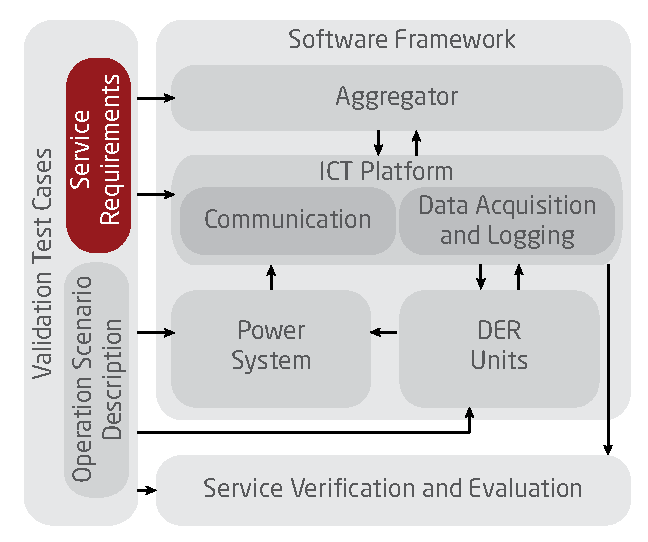
\includegraphics[width=\textwidth]{framework_services.eps}
	\caption{This chapter focuses on the \emph{service definition} block of the aggregator validation framework presented in Chapter~\ref{cha:validation}.}
      \label{fig:framework_services}
\end{marginfigure}

\newchapter{T}{he requirements for ancillary} services in many countries are defined, due to historical reasons, on the assumption that only generators provide ancillary services. It is clear that current service requirements in many countries are directly, or indirectly, blocking the integration of aggregators providing DR\fcite{cappers2013assessment,coalition2014mapping}. If aggregators are to be successfully integrated into the power system, the rules and requirements for participation must be changed. This chapter presents two novel contributions to integrating aggregators in the power system: a modeling method for services, and a proposal for the restructuring of requirements for ancillary services. A method for modeling services is important because the resulting models form the benchmark for the performance evaluation and verification of the aggregator (see Chapter~\ref{cha:verification}), as well as being a direct input to the aggregator (see Chapter~\ref{cha:aggregator}). The redefinition of ancillary service requirements is important since it will allow system operators to utilize the properties of all available resources, both traditional and new, in an optimal way. 

The concepts presented in this section are part of two draft journal papers\fcite{bondy2016method,bondy2016redefining} which can be found in Appendix~\ref{app:segan} and Appendix~\todo{Berkeley Ref}, as well as work done as a collaborating author for a conference paper\fcite{heussen2013a} and a technical report written for the iPower consortium\fcite{bondy2014flech}. Section~\ref{sec:backgroundservicesandreq} discusses different kinds of services that aggregators can provide and Section~\ref{sec:modelingAS} presents how these can be modeled. These models are directly related to the \emph{service requirements} block in the aggregator validation framework (see Figure~\ref{fig:framework_services}). In Section~\ref{sec:RedefiningAncillaryServiceRequirements} a proposal for how ancillary service requirements can be reformulated in order to be technology agnostic. 

%Content of this chapter is the work done at LBNL and through the iPower demo.
%\begin{itemize}
%	\item Service definition
%	\item What are aggregators expected to deliver?
%	\item PowerMax service requirements
%	\item Redefining Ancillary Services Requirements for Technology Agnostic Resources
%\end{itemize}

\section{Background}\label{sec:backgroundservicesandreq} % (fold)
\newsection{T}{he following section outlines} concepts related to the definition and requirements of services at TSO and DSO level. While services for the TSO (ancillary services) are well established, DSO services are a relatively new concept which has been explored in iPower project\fcite{ipower2013development}.
\subsection{What are Ancillary Services?} % (fold)
\label{sub:ancillaryservicesdef}
Defining what \gls{as} are, as well as which services the term includes, is difficult. This is due to both the differences in the way power systems are managed around the world and the differences in the terminology used to refer to such services. There is overlap between the European and US definition\fcite{eurelectric2004,ferc1997} of AS in that both describe them as services used to ensure the reliability of the power system. In both European and US context reliability is addressed by considering \emph{system adequacy} and \emph{security} \footnote{NERC also used the term system security, but in September 2001 security became synonymous with homeland protection in the US. Now it uses the term \emph{operating reliability} \cite{nerc2007definition}}. \emph{System adequacy} is the power system's ability to supply the electricity demand at all times and \emph{security} is the ability to withstand sudden disturbances.

Generally, maintaining an adequate and secure power system means maintaining the power system operating at nominal frequency and voltage. In cases where the power system deviates from nominal operation, either due to natural fluctuations in production/consumption or faults in the system, the system operators will activate ancillary services to restore normal operation. 

Some countries, \eg Denmark, consider voltage control, black start capabilities, short circuit control and reactive reserves as AS. This work focuses on those services that use active power to maintain the nominal frequency of the grid. In Europe\footnote{ENTSO-E changed in 2013 its nomenclature of AS, and the three presented here correspond roughly to the classical primary, secondary and tertiary reserves as presented in \cite{Rebours}.} these services are \glspl{fcr}, \glspl{frr} (either automatic\footnote{In the United States, regulation is used for system balancing. This service corresponds to automatic FRR.} or manual), and \glspl{rr}\fcite{entsoe2013network}.

These reserves are activated as illustrated in Figure~\ref{fig:MAINfreqcont}. The FCR is the fastest reserve and reacts automatically upon the grid measurements. Its role is to stop frequency excursions and its effectiveness can be measured by the \emph{frequency nadir} \cite{eto2010use}. The FRR is activated by tracking the \gls{agc} signal, or through manual activation by the system operator, relieves the FCR (allowing the FCR to be available again) and restores the frequency to the nominal value. The RR relieve the FRR, usually through rescheduling of units or by bringing inactive units online.

\begin{figure}[htbp!]
\centering
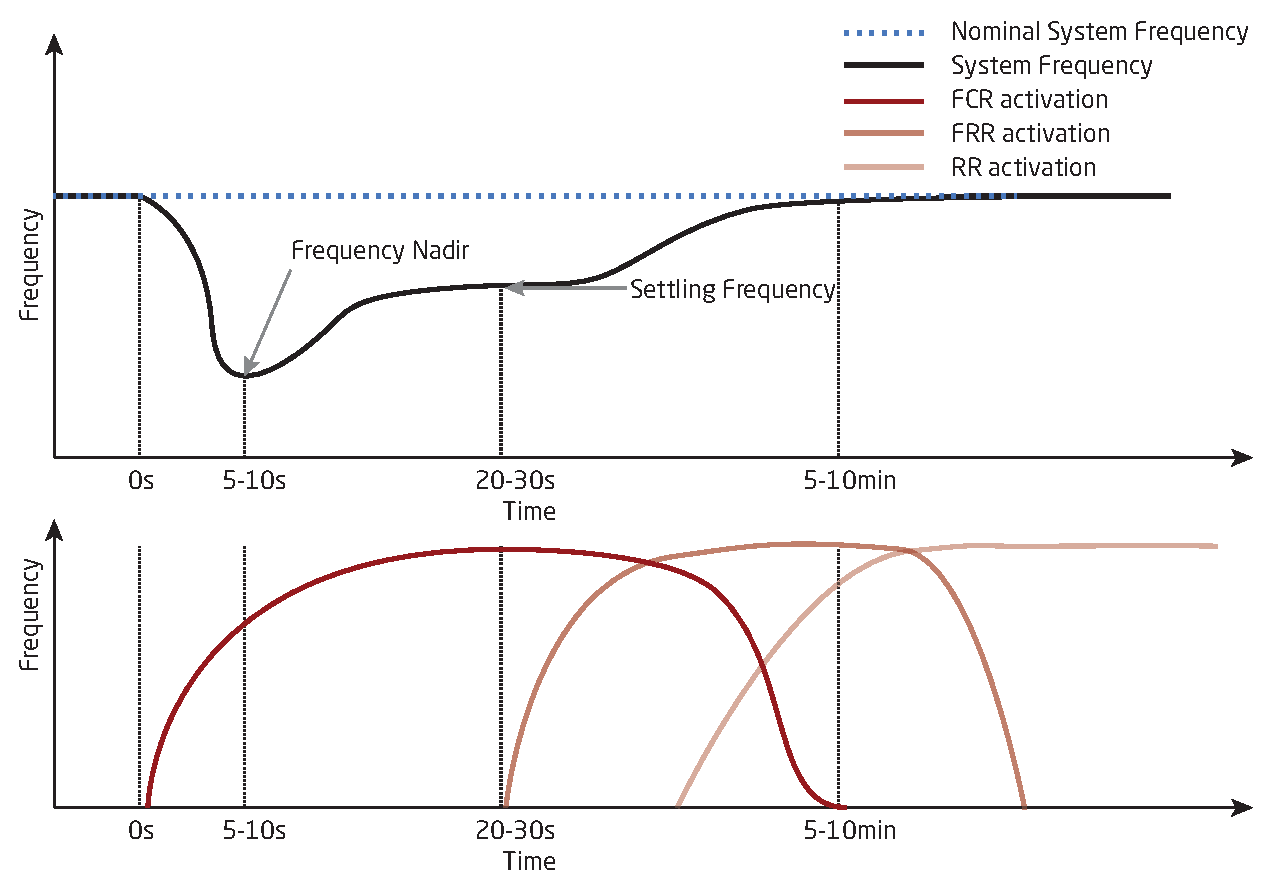
\includegraphics[width=0.9\textwidth]{frequency_contingency.eps}
\caption{The ancillary services are activated sequentially after a frequency contingency. In systems with high inertia the frequency nadir will occur at frequencies closer to the nominal frequency.}
\label{fig:MAINfreqcont}
\end{figure}

% subsection What are Ancillary Services? (end)
\subsection{Requirements for Ancillary Services} % (fold)
\label{sub:servreqAS}
Because AS are essential for the secure operation of the system, the system operators have requirements and restrictions on the units providing AS. A super-set of requirements across different systems was presented by \emph{Rebours}\fcite{Rebours}, and following his overview we classify requirements into three categories:
\begin{description}
	\item[temporal requirements] which relate to how fast and for how long a service must be delivered;
	\item[resource tuning requirements] which relate to specific values that tuning parameters in the resource must have;
	\item[market requirements] which relate to bid sizes and similar parameters in systems where services are acquired through market mechanisms.
\end{description}

Of these three categories, only the temporal requirements relate to service performance. Furthermore, in most systems, the requirements are implicitly defined for traditional generation units. This means that most service requirements are oriented towards the least common denominator of service providers, e.g. a unit providing FCR should provide half of the service within 15 seconds and full response within 30 seconds\fcite{EnerginetAncillary}. A variety of generation and consumption units would be able to provide this service faster, but this quality is not rewarded. Another example is the requirement of having a PI-controller on units providing FRR in order to track the AGC signal. Such a controller is infeasible on distributed systems, but other modern controllers can provide offset-free control with similar properties. This means that the historical requirements for units participating in AS markets in many countries act implicitly, or explicitly, as barriers for new technologies to enter the market\fcite{cappers2013assessment,coalition2014mapping}.%\todo{should I put in a more thorough description of FCR, FRR and RR, like what we have in the DDRAS paper?}

The concept of using demand side management to help the secure operation of the power grid has existed in different forms since the late 1970s\fcite{lampropoulos2013history}. But in recent years, the introduction of new consumption and generation technologies, \ie DERs, along with the roll-out of a smart metering infrastructure and the advances in ICT, has lead to the new opportunities in using smart control of small scale consumption/production as a service to the power grid. There is a large body of literature\fcite{oconnell2014benefits} concerning DR, and proposals to use it for AS\fcite{vrettos2015integrating,mathieu2012using,zarogiannis2014dynamic}.%\clearpage
% subsection Service Requirements for Ancillary Services (end)
\subsection{Distribution System Services} % (fold)
\label{sub:dsoservices}
As the amount of DERs installed at distribution level increases, the DSOs face new operational problems. Mainly, the increase in electric load will cause congestion and voltage issues. The traditional way of handling these are through reinforcement of the grid assets. Given the high cost of installing new cables, and the uncertainty in how the electricity consumption will change in the future, the use of flexibility services will be an attractive alternative.

One of the main outcomes of the iPower project was the definition of a set of flexibility services that demand aggregators can provide DSOs\fcite{ipower2013development} for congestion management or voltage issues. The requirements for three of the congestion management services have been further detailed individually\footnote{The services requirements were detailed in the following technical reports\cite{hansen2013flech,biegel2014flech,bondy2014flech}.}, and aggregator architectures have been designed to provide both congestion management\fcite{hu2014coordinated} and voltage support\fcite{han2014assessment}. At the same time, the concept of the \gls{flech} has been designed as a platform to enable the transparent contracting of flexibility\fcite{heussen2013a}.

An example of a flexibility service is the \emph{PowerMax}\fcite{bondy2014flech} service, where the aggregator maintains the total consumption of its portfolio under a limit, within a specified period of time. This means that the aggregator is free to manipulate its portfolio as long as its peak load is below the limit specified by the DSO.
% subsection DSO Services (end)
\subsection{Asset Management Services} % (fold)
\label{sub:assetmanagementservices}
In Chapter~\ref{cha:aggregator} the concept of \gls{ams} is introduced as the services that an aggregator provides to the owner of the DERs, or flexibility assets. An example of this is the case where the aggregator is an EV fleet operator that has the contractual responsibility of maintaining all EVs in the fleet within a certain \gls{soc}. The purpose of validating aggregators for these services is that flexibility asset owners can use the validation as a trust measure.

The main idea behind AMS is that the flexibility assets have a primary purpose, which is to satisfy the needs of their owner. The aggregator can use the flexibility of the units as long as the primary purpose is respected. Thus, from the perspective of customer comfort, an aggregator that is better at AMS is more desirable. 
% subsection Asset Management Servc (end)
% section Background on Aggregator Services (end)
\section{Modeling of Service Requirements} % (fold)
\label{sec:modelingAS}
\newsection{T}{he validation framework} presented in Chapter~\ref{cha:validation} uses the \emph{service requirements} as a benchmark towards which the aggregator is evaluated. This is because the requirements form the control objective of the aggregator. Currently, requirements for services are encoded within the contractual agreements between system operator and service provider. A standard method is needed for extracting this information and building a model that can be used for benchmarking.

By analysing the services presented in Section~\ref{sec:backgroundservicesandreq}, a method for translating the contracts into a time series model has been developed. The method consists of the following six steps:
%form have been identified as a generic method for modeling ancillary services. The steps are exemplified by DSO services defined in  and TSO services defined in :
\begin{enumerate}
  \item Identify physical parameters defining the service.
  \begin{itemize}
    \item \eg Power production or consumption, measured grid frequency, time measurements, etc.% Including maximum measuring sensitivities.
  \end{itemize}
  \item Identify the dynamic behaviors of the service related to system parameters (if any).
  \begin{itemize}
    \item \eg FCR expects a linear relation between a deviation from the nominal grid frequency and the generator set-point.% Power-cap has a dynamic relationship between feeder load and the controllable load power in order to keep the total feeder load at a $P_{DSO,Ref}$ value.
    %\item PowerMax is not dynamic. The aggregator must control $\Delta P_{Agg}$ to ensure that he does not violate $P_{max,Agg}$. But the service does not require a dynamic behavior related to a system parameter like primary frequency regulation and PowerCap.
  \end{itemize}
  \item Identify the physical size of the service and the tolerated error. % Both ideal service and minimum required service.
  \begin{itemize}
    \item \eg the volume of the bid for FCR. %Physical size is for example $P_{max,Agg}$ for PowerMax service or
%    \item Tolerance is for example $P_{max,Agg}+P_{tolerance}$ for the PowerMax service and allowed dead-band for DK1 primary reserve.
  \end{itemize}
  \item Identify the ideal response time of the service and acceptable response.
  \begin{itemize}
%    \item Most contracts comes with some timing specifying how fast the service provider must act.
    \item \eg FCR in western Denmark must be 50 \% of activated within 15 s and 100 \% within 30 s.
%    \item The ideal service is for example an instantaneous step in power to 100 \% of set-point for DK1 primary reserve.
  \end{itemize}
  \item Based on the dynamics, size and timing of the service, as well as the tolerated errors from points 1--4, develop a time series for ideal and acceptable service provision. The model will be a set of time series: $\mathbf{x}_{ideal}(t)$ for ideal response and $\mathbf{x}_{acc}(t)$ for acceptable response. Both time series can be a scalar or a vector, e.g. $\mathbf{x}_{acc}(t)$ can be formed by a set of upper and lower tolerance bounds or simply by an upper bound.
  \item Identify how the service error is to be measured.
\end{enumerate}

  %§$\mathbf{x}_{ideal}(t)$ and $\mathbf{x}_{acc}(t)$ can be a pair of values, e.g. minimum and maximum tolerance limits, for some services and may be only a single value, e.g. minimum or maximum tolerance, for others. 
Furthermore, the analysed services can be divided into three kinds of services:
\begin{description}
	\item[Reference Tracking:] Services where a reference signal must be followed, \eg regulation in the United States.
	\item[Band Service:] Services where the output is able vary between an upper and lower limit, \eg smart charging of a fleet of EVs.
	\item[Cap Service:] Services where the output must respect either a upper or lower bound, \eg the \emph{PowerMax} service.
\end{description}

Based upon the three kinds of service, the service error can be measured the following ways:
\subsection*{Reference tracking}

Reference tracking error can be calculated as:
\begin{equation}\label{MAINeq:ref_error}
e(t) = x_{meas}(t) - x_{ideal}(t),
\end{equation}
\begin{marginfigure}
	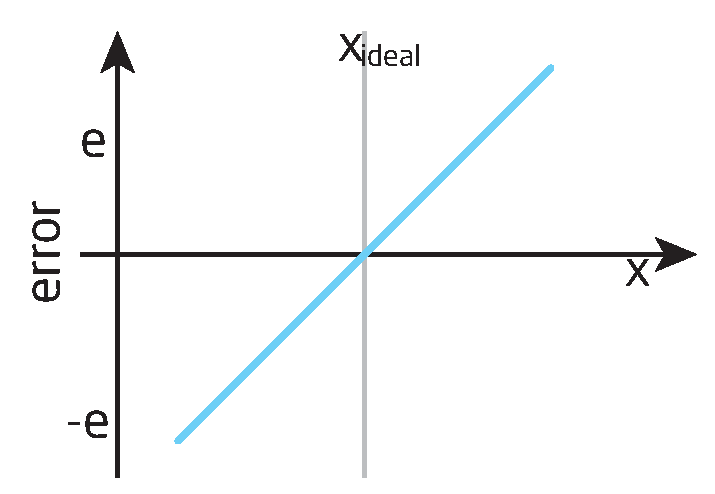
\includegraphics[width=\textwidth]{tracking_error2.eps}
	\caption{Error in reference tracking.}
      \label{fig:reftrackerrorMAIN}
\end{marginfigure}
where $x_{meas}(t)$ is the measured output, \eg the total load of the aggregator portfolio, and $x_{ideal}(t)$ is the ideal response defined in the service model. This definition will lead $e<0$ for measured values below the ideal and $e>0$ for values above the ideal. In this case $\mathbf{x}_{acc}(t)$ will be a band around $x_{ideal}(t)$, and the values of $\mathbf{x}_{acc}(t)$ do not need to be symmetric.

\subsection*{Band service}
The ideal response in a band service is defined as $ \mathbf{x}_{ideal}(t)= [x_{min}(t),x_{max}(t)]$. The error in the band service can therefore be estimated by:
\begin{equation}\label{MAINeq:band_error}
e(t)=
\begin{cases}
x_{meas}(t) - x_{min}(t) , & x_{meas}(t) < x_{min}(t)  \\
0, & x_{min}(t) \leq x_{meas}(t) \leq x_{max}(t) \\
x_{meas}(t) - x_{max}(t), & x_{meas}(t)  > x_{max}(t).  
\end{cases}
\end{equation}
\begin{marginfigure}
	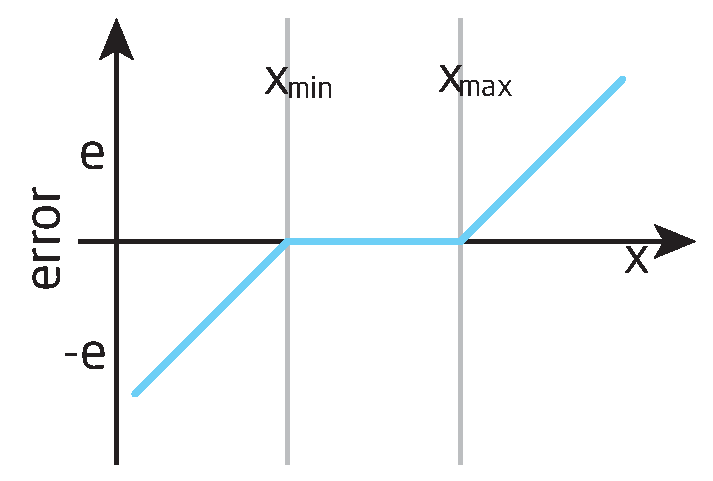
\includegraphics[width=\textwidth]{band_error2.eps}
	\caption{Error in band service.}
      \label{fig:banderrorMAIN}
\end{marginfigure}

In this case, the $\mathbf{x}_{acc}(t)$ is a set of values that surrounds the band defined by $ \mathbf{x}_{ideal}(t)$, as seen in Fig.~\ref{fig:RefErr}. The values of $\mathbf{x}_{acc}(t)$ do not need to be symmetric around the band.

\subsection*{Cap service}
%Maximum/minimum cap error only counts the error when performance is above/below some ideal value. 
In cap services, error is only tracked when $x_{meas}(t)$ is either above or below a given a limit value.
Maximum cap error is calculated as shown in \eqref{MAINeq:maxmin_cap} and minimum cap can be similarly calculated. In \eqref{MAINeq:maxmin_cap}, $x_{max}(t)$ is the ideal maximum limit according to the service contract:

\begin{equation}\label{MAINeq:maxmin_cap}
e(t)=
\begin{cases}
x_{meas}(t)-x_{max}(t), & x_{meas}(t) > x_{max}(t) \\
0, & x_{meas}(t) \leq x_{max}(t).
\end{cases}
\end{equation}
\begin{marginfigure}
	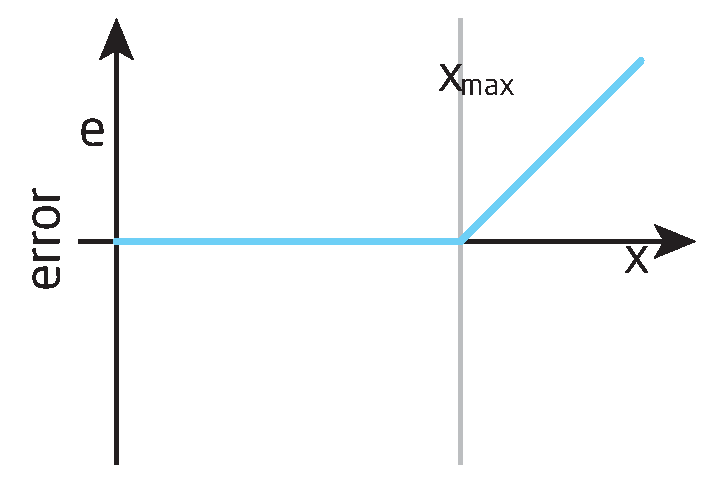
\includegraphics[width=\textwidth]{cap_error2.eps}
	\caption{Error in cap service.}
      \label{fig:caperrorMAIN}
\end{marginfigure}

In the cap service, $x_{acc}(t)$ is a limit that either lies below $x_{min}(t)$ or above $x_{max}(t)$.


% section Modeling of Ancillary Services (end)

%
\section{Restructuring Ancillary Service Requirements} % (fold)
\label{sec:RedefiningAncillaryServiceRequirements}
Until now, system operators have been able to arrest frequency excursions fast enough because of the inherent system inertia. With the increasing penetration of wind power in the system, the electricity prices are lowered and operating fossil-fueled generator becomes economically unfeasible. This has the effect of reducing the system inertia, and reducing the availability of AS resources. Therefore new AS sources with faster response times are required. \emph{Vrettos et al.}\cite{vrettos2015integrating} show that if FCR is provided by DR (with a very fast response), the frequency nadir occurs at higher frequencies.
Also, \emph{Makarov et al.}\cite{makarov2008assessing} argue that the value of regulation resources can be defined based upon the ramp capabilities of the service providing units. Faster reacting units are more valuable to system operators, since they help arrest the frequency excursion faster and at a higher nadir.% It does require changes to the AGC in order to utilize the fast response, but this would also lead to the need for fewer reserves.

AS requirements are specified by a system operator based on the desired control response for a particular power system, under the implicit assumption that the ideal unit response corresponds to a scalar fraction of the required system response. Today, these requirements --- as reflected in the service definition --- are not differentiated according to the capabilities of the unit providing the service. Therefore, service definitions are designed to accommodate the least capable unit in the portfolio. As a consequence, more capable units are not being fully utilized, leading to excess contracting of service providers.

 In this section a new form of defining AS requirements is presented, which has as an objective to allow all units to participate in the AS markets on equal footing. The main assumption is that all units can be valuable for AS provision, even when they do not fully comply with current requirements, and that the system operators will be able to manage the system better if the capabilities of all available resources are utilized. Also, units should be remunerated based upon the value they represent to the operation of the system, and their performance compared to these expected values.

Regulative authorities have concluded that fast reacting units are valuable for the system operation, and started programs to benefit of these resources. An example of this is FERC order 755 (Pay for Performance) which has led to PJM splitting their regulation market product into RegA, for slow reacting units, and RegD for fast reacting units. The product differentiation approach has been a success for PJM, but  splitting the market may still lead to suboptimal utilization of units and does not address the issue of new technologies being effectively excluded from certain markets.  We propose instead to restructure the ancillary service definitions such that all types of service providers participate with the same market product defined by a set of optimal performance parameters, and not by minimum requirements. This means that the all entities providing a given ancillary service are optimally cleared under a single market.

\subsection{The Overall Approach} % (fold)
\label{sub:TheOverallApproach}
The restructuring of AS requirements is formed by the following key concepts:
\begin{enumerate}
	\item The system operator is able to formulate an overall \emph{ideal AS response} that can be achieved through an optimal mix of resources. Any resource can make a bid for providing part of this ideal response.
	\item The \emph{parametrization of AS bid}, where the parameter values of each unit/bid reflect the service provider's capabilities to partially fulfill the ideal response. This avoids excluding units that may have useful capabilities in one parameter, e.g. very fast ramp rate, but low capabilities in another parameters, e.g. only holding the response for a short time. Such a service definition allows compliance to be measured on a linear rather than a binary scale: In addition to compliance and noncompliance, different levels of partial compliance are possible.
	\item Clearing all units under a \emph{generalized single clearing-price auction} allows constructing an optimal portfolio, and enables competition between all resources, leading to lower prices.
    \item \emph{Performance-based remuneration} gives incentive to better AS provision and enables transparent performance-based clearing of the market.
\end{enumerate}

These key concepts are discussed individually in the following subsections.
% subsection The Overall Approach (end)
\subsection{Ideal Service Tender} % (fold)
\label{sub:IdealServiceTender}
The ideal source for AS is one with ``unlimited capabilities in terms of response time, energy output, ability to frequently reverse their output, ability to respond and follow the AGC setpoint changes, and size .''\cite{makarov2008assessing}\footnote{For this kind of response to be optimal, changes must be made to the AGC algorithm \cite{peydayesh2012effects}.} It is impossible for any one unit to possess these characteristics, but system operators aim at achieving this kind of system response by contracting several units.

For example, a system operator could determine that the ideal system response to a frequency excursion is the one that has a resulting frequency nadir at the settling frequency (thus minimizing the risk of tripping the under-frequency relays). Based upon the inertia in its system, the system operator determines the volume ($V_{tot}$) needed as well as the response characteristics needed to achieve this, see Figure~\ref{fig:idealresponse}.

\begin{figure}[htbp!]
\centering
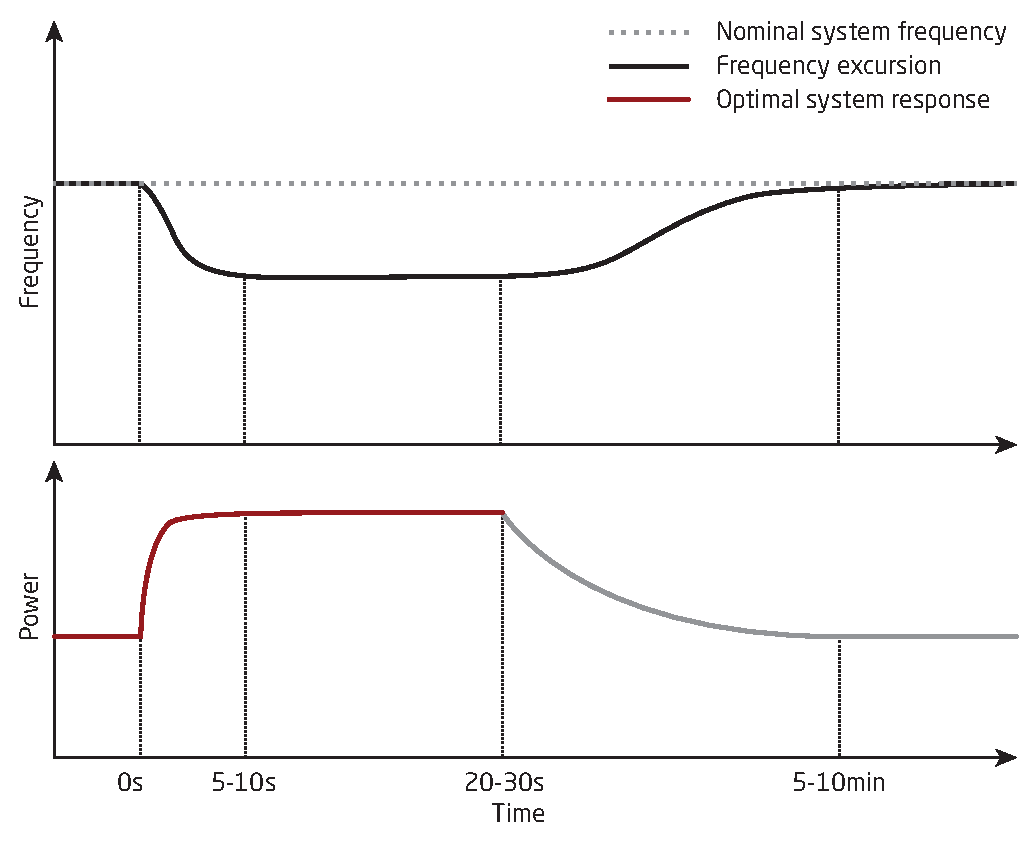
\includegraphics[width=0.9\columnwidth]{primary_frequency_control_ideal.eps}
\caption{In this case, the ramp of the ideal response is mainly determined by the system inertia and is to be sustained until FRR can be activated.}
\label{fig:idealresponse}
\end{figure}
% subsection Ideal Service Tender (end)
\subsection{Service Parametrization} % (fold)
\label{sub:ServiceParametrization}
The overall ideal service requirements can be expressed as:
\begin{equation}
	S^* = f_m(\textbf{x}^*) \label{eq:optimaltender}
\end{equation}
where $\textbf{x}^*$ is a vector of ideal parameter values and $f_m(\cdot)$ a function that translates the parameters $\textbf{x}$ into a model, e.g. into a time series as shown in Section~\ref{sec:modelingAS}. Furthermore, the system operator must inform how the parameters are valued with respect to the $S^*$, which is done through a capability value:
\begin{align}
    \kappa &= g(\mathbf{x}) \\
    \kappa &\in [0,1].
\end{align}

For example, a system operator decides that FCR in their market is defined by $\textbf{x} = [\tau_r,\tau_d,V]$, where $\tau_r$ is the rise time of the service, $\tau_d$ is the duration of the service, and $V$ is the volume of the service. Due to the properties in its system, it decides that $\textbf{x}^* = [30 s, 20 min, 90 MW]$. The capability value of each bidder is calculated by:
\begin{equation}
	\kappa_i = \alpha_1 \frac{\tau_{r,0}}{\max({\tau_{r,0},\tau_{r,i})}} + \alpha_2  \frac{\min(\tau_{d,0},\tau_{d,i})}{\tau_{d,0}} + \alpha_3 \frac{V_i}{V_{tot}}, \quad \forall \, i \in \Omega \label{eq:kappa_primfreq}
\end{equation}
where $\tau_{r,0}$ and $\tau_{d,0}$ are a nominal value the system operator sets, $\tau_{r,i}$ and $\tau_{d,i}$ are the actual parameter values for each bidder, $\frac{V_i}{V_{tot}}$ is the bid contribution to the total required volume, and $\Omega$ is the pool of bids. Finally, $\sum_{i} \alpha_i = 1$, and in this case could be $\alpha_1,\alpha_2 = \frac{2}{5}, \alpha_3 = \frac{1}{5}$.
% subsection Service Parametrization (end)

\subsection{Market Mechanism} % (fold)
\label{sub:MarketMechanism}
It is impossible to restructure the AS definition without addressing the market mechanism for determining the optimal set of resources. The market should be designed as a single clearing price auction, in which each resource bid is adjusted by \emph{two} factors for bid quality: 1) the capability value $\kappa_i$ and 2) a historical performance\footnote{The historical performance parameter can also be interpreted as an availability parameter, or certainty parameter.} parameter $\eta^{hist}_i$. In this section a proposal for how this market mechanism could be formulated is presented.

The proposed clearing mechanism identifies a common clearing price based on the most expensive accepted bid\footnote{This is similar to the merit order lists used in \eg the Nordic system for Manual Regulating Power\cite{bondy2013}.}:
%Clearing principles
\begin{equation}
    P^\mathtt{clear} = \max P^\mathtt{bid}_i, \quad i \in \Omega^\mathtt{acc}
\end{equation}
where $\Omega^{acc}\subseteq \Omega$ is the subset of accepted bids of the set of received bids $\Omega$. 
The clearing mechanism selects the subset of bids which offer the cheapest overall clearing cost and meet the tender requirements with a given certainty of availability: 
\begin{align}
      \Omega^\mathtt{acc} &= &\mathtt{argmin}_{\Omega^\mathtt{hyp} \in \mathcal P(\Omega)} \sum_{i\in \Omega^\mathtt{hyp}}{\kappa_i P^\mathtt{clear}_i } & \\
	  &\mathtt{s.t.}& \sum_{i\in \Omega^\mathtt{hyp}} f_m(\mathbf{x}) \geq S^* &  \\
      &~ & \eta^{hist}_i \geq \eta^{hist}_{min} &\quad \forall \, i \in \Omega^\mathtt{hyp} 
\end{align}
Where $\mathcal P(\Omega)$ denotes the Power Set of $\Omega$ and $\Omega^{hyp}$ is a subset of the Power Set. $S^*$ is the ideal tender from Eq.~\eqref{eq:optimaltender} and $\eta^{hist}_{min}$ is the minimum historical performance requirement to participate in the market\footnote{This value represents how averse the system operator is to risk, and could also be considered part of the service parameters $\textbf{x}$.}.

% subsection Market Mechanism (end)

\subsection{Performance Based Remuneration} % (fold)
\label{sub:PerformanceBasedRemuneration}

The estimation of the service provision performance can be done in different ways, depending on which parameters the system operator deems to be the most critical. The concept of performance assessment is discussed in Chapter~\ref{cha:verification}, and performance index is introduced there. Here it suffices to say that the performance measurement is a function of the error in service delivery:
\begin{align}
	\eta &= c(e(t)), \label{eq:perfindexsimple}\\
	\eta &\in [0,1]
\end{align}

We propose that remuneration is based on the performance evaluation of the service provision:
\begin{equation}
	P^\mathtt{rem}_i = \eta_i\kappa_i  P^\mathtt{clear} \qquad \forall \, i \in \Omega^\mathtt{acc}.
\end{equation}
Thus, remuneration is based upon the value the resource has to the grid operator, how well it performs, and the most expensive activated resource.
% subsection Performance Based Remuneration (end)

% section Redefining Ancillary Service Requirements (end)

\section{Conclusions on Service Requirements} % (fold)
\label{sec:ConclusionsServiceRequirements}
\newsection{A}{ggregators have become} possible sources for ancillary services and distribution system services. While system operators are aware of the potential in using flexibility for system balancing, the ancillary service requirements have not been changed in order to accommodate this new technology. This chapter presented a novel proposal for solving this issue, by restructuring the ancillary service requirements based upon a set of optimal parameters instead of the limiting minimum requirements found in many systems today.

Also, a method for modeling services was shown. The resulting models are relevant for the validation framework in that they provide the benchmark towards which aggregators must perform. In Chapter~\ref{cha:verification} it is shown how the service models can be used for performance assessment and verification of services.

The work presented in this chapter differs from the rest of the thesis, in that the concepts presented here are not focused on the aggregator itself. The service modeling method can be applied to any kind of service, not necessarily those provided by aggregators, and the objective of the ancillary service restructuring is to include any new technology, not only aggregators providing DR.

A final observation with respect to services is that operators like Energinet.dk are interested in acquiring flexibility from aggregators. The traditional approach to buying ancillary services is that the operator pays for an increase or decrease in power production, but flexibility has an extra dimension: time\footnote{See Chapter~\ref{cha:aggregator}.}. That is, flexibility is not only about increasing and decreasing production, but also about moving it in time. System operators expect flexibility services to fit in within the existing framework, but the two kinds of services can arguably be said to be essentially different. 

% section Conclusions on Service Requirements (end)
% chapter Service Requirements (end)
